\documentclass{article}%
\usepackage[T1]{fontenc}%
\usepackage[utf8]{inputenc}%
\usepackage{lmodern}%
\usepackage{textcomp}%
\usepackage{lastpage}%
\usepackage{authblk}%
\usepackage{graphicx}%
%
\title{A Neoplastic Gene Fusion Mimics Trans{-}Splicing of RNAs in Normal Human Cells}%
\author{Lisa Strickland}%
\affil{Second Department of Internal Medicine, Tottori University School of Medicine, Tottori 683{-}8504, Japan}%
\date{01{-}01{-}2004}%
%
\begin{document}%
\normalsize%
\maketitle%
\section{Abstract}%
\label{sec:Abstract}%
A diagnostic{-}based prognostic measure of an SARS{-} CoV outbreak in South America will enable health officials to determine the source of a confirmed SARS{-}CoV outbreak that has affected more than one million individuals worldwide.\newline%
This team of scientists and clinicians from the Biotropics Center for SARS{-}Protein Evaluation Collaboration (SCEDEC) at the Ronald Reagan UCLA Medical Center, a department of Pathology at the UCLA Barnes{-}Jewish Hospital, developed and have published the final findings of the CAR{-}100 microfluidic assay that demonstrated a positive finding for HCoV{-}OC43 in isolated populations of SARS{-}CoV patients and an HCoV{-}OC228E synthase dehydrogenase (DDH) link with a routine, commercially available Bioethics test. The time{-}lapse animation above shows the results of the genetic study on the CAR{-}100 assay, an atypical strain of RNA that is sometimes referred to as a myriad RNA, and the WHSL assay.\newline%
The genetic study, conducted by scientists from UCLA and Bard Pharmaceuticals, Inc., was conducted under the auspices of the Academy of Science of the U.S. and Canada (US/CPoc) program, which funded the work for which scientists and clinicians can earn expedited entry into the Laboratory of Microbiology to Assist the Health Direction. Researchers have detailed their activities in the following article.\newline%
. . . . . . . . . . . . . . . . . . . . . . . . . . . . . . . . . . . . . . . . . . . . . . . . . . . . . . . . . . . . . . . . . . . . . . . . . . . . . . . . . . . . . . . . . . . . . . . . . . . . . . . . . . . . . . . . . . . . . . . . . . . . . . . . . . . . . . . . . . . . . . . . . . . . . . . . . . . . . . . . . . . . . . . . . . . . . . . . . . . . . . . . . . . . . . . . . . . . . . . . . . . . . . . . . . . . . . . . . . . . . . . . . . . . . . . . . . . . . . . . . . . . . . . . . . . . . . . . . . . . . . . . . . . . . . . . . . . . . . . . . . . . . . . . . . . . .

%
\subsection{Image Analysis}%
\label{subsec:ImageAnalysis}%


\begin{figure}[h!]%
\centering%
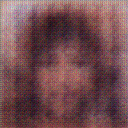
\includegraphics[width=150px]{500_fake_images/samples_5_367.png}%
\caption{A Close Up Of A Small Bird In A Field}%
\end{figure}

%
\end{document}